\documentclass[runningheads]{ctexart}
\usepackage{graphicx}
\usepackage{booktabs}
\usepackage{amsmath}
\usepackage{float}
\usepackage{hyperref}
\usepackage{xcolor}
\usepackage{listings}

% --- 中文支持 / Chinese Support ---
\renewcommand{\abstractname}{摘要}
\renewcommand{\contentsname}{目录}
\renewcommand{\figurename}{图}
\renewcommand{\tablename}{表}
\renewcommand{\refname}{参考文献}
\newcommand{\keywordsname}{关键词}
% ---------------------------------

\lstset{
    language=Python,
    basicstyle=\ttfamily\small,
    keywordstyle=\color{blue!70!black},
    commentstyle=\color{green!40!black},
    stringstyle=\color{orange!60!black},
    showstringspaces=false,
    breaklines=true,
    frame=single,
    tabsize=4
}

\begin{document}

\title{深度学习实践 1 - 图像分类算法对比}
\author{李祥熙 2234412799}
\date{2026年4月30日}

\maketitle

\begin{abstract}
本实验针对 CIFAR-10 图像分类任务，使用 PyTorch 编写了卷积神经网络（CNN）并在不同学习率和 epoch 下进行训练，同时使用 scikit-learn 实现了随机森林（Random Forest）算法并在不同决策树数量下进行了对比。对两种算法在准确率（Accuracy）、精确率（Precision）、召回率（Recall）、F1-score 以及训练和测试时间等指标上进行了全面评估，系统地比较了深度学习算法与传统机器学习算法在图像数据上的优劣。

\vspace{10pt} % 增加间距
\noindent \textbf{\keywordsname：} 卷积神经网络 \and 随机森林 \and 深度学习 \and 图像分类 \and CIFAR-10
\end{abstract}

% --- 正文部分 ---
\section{实验目的}
本实验的目标如下：
\begin{itemize}
    \item 目标一：掌握前馈神经网络和卷积神经网络（CNN）的基本原理，使用 PyTorch 框架自行编写简单的 CNN 模型并进行图像分类训练。
    \item 目标二：复习传统机器学习算法，使用 scikit-learn 库调用随机森林算法在同样的图像数据集上进行分类训练。
    \item 目标三：对比 CNN 与 Random Forest 在不同参数配置下的准确率、精度、召回率、F1-score，同时测量记录两者在训练过程和推理过程的耗时，通过定量化的实验数据深刻理解深度学习相对传统算法的优势与不足。
\end{itemize}

\section{实验原理}
\subsection{卷积神经网络（CNN）}
CNN 通过局部感受野与权重共享机制学习空间相关性特征。卷积层输出的特征图经过非线性激活函数（如 ReLU）引入非线性表达能力，再通过池化层进行空间下采样以提升平移不变性并减少参数规模。最终使用全连接层完成类别映射，从而实现端到端的图像分类。

\subsection{随机森林（Random Forest）}
随机森林是一类基于 Bagging 的集成学习方法，通过对不同子样本训练多棵决策树并进行投票或平均来得到最终预测。其优势在于训练速度快、对超参数不敏感且易于并行化，但对高维、结构化空间特征的表达能力不足。因此在图像分类任务中通常性能弱于 CNN。

\subsection{指标与评价策略}
本实验使用 Accuracy 评估整体分类准确度，并使用宏平均的 Precision、Recall 和 F1-Score 体现类别均衡情况下的综合表现。宏平均对每个类别等权，避免少数类被忽略。时间开销分别统计训练与测试阶段，以体现“性能-效率”之间的取舍。

\section{实验过程}
\subsection{实验环境}
\begin{itemize}
    \item 操作系统：MacOS
    \item 编程语言：Python 3
    \item 深度学习框架：PyTorch (结合 torchvision)
    \item 其他关键工具：scikit-learn, NumPy, pandas, Matplotlib
\end{itemize}

\subsection{数据集与预处理}
\begin{itemize}
    \item 数据集名称：CIFAR-10 数据集。该数据集包含 60000 张 32x32 分辨率的 RGB 彩色图像，划分为 10 个类别（每类 6000 张）。其中 50000 张用于训练，10000 张用于测试。
    \item 数据特征：输入维度为 $[3, 32, 32]$ 的张量。
    \item 预处理步骤：
    \begin{itemize}
        \item 对于 CNN，将图像使用 \texttt{transforms.ToTensor()} 转换为 Tensor 后，使用 \texttt{transforms.Normalize((0.5, 0.5, 0.5), (0.5, 0.5, 0.5))} 缩放到 \([-1, 1]\) 区间。
        \item 对于随机森林等传统方法，需要先将 $[N, 3, 32, 32]$ 的多维张量展平（Flatten）为二维特征矩阵 $[N, 3072]$ 以满足 sklearn 接口需求。
    \end{itemize}
\end{itemize}

\section{实验内容}
\subsection{任务一：CNN 模型构建与训练}
基于 PyTorch 自行搭建的 CNN 包含两个卷积层和最大池化层，接着通过全连接层输出分类结果。输入为 $[3, 32, 32]$ 的图像张量，经过两次卷积与池化后，特征图尺寸变为 $[32, 8, 8]$，再展平进入全连接层得到 10 类输出。分别使用 $lr=0.001, epoch=5$、$lr=0.001, epoch=2$、$lr=0.01, epoch=5$ 的不同配置进行优化器（Adam）超参数评估，核心损失函数选用 \texttt{CrossEntropyLoss}。

\begin{lstlisting}
class SimpleCNN(nn.Module):
    def __init__(self):
        super().__init__()
        self.conv1 = nn.Conv2d(3, 16, kernel_size=3, padding=1)
        self.pool1 = nn.MaxPool2d(2, 2)
        self.conv2 = nn.Conv2d(16, 32, kernel_size=3, padding=1)
        self.pool2 = nn.MaxPool2d(2, 2)
        self.fc1 = nn.Linear(32 * 8 * 8, 256)
        self.fc2 = nn.Linear(256, 10)

    def forward(self, x):
        x = self.pool1(F.relu(self.conv1(x)))
        x = self.pool2(F.relu(self.conv2(x)))
        x = x.view(-1, 32 * 8 * 8)
        x = F.relu(self.fc1(x))
        return self.fc2(x)
\end{lstlisting}
    上述代码展示了网络的整体结构：两层卷积分别提取低级与中级特征，池化层将空间尺寸减半以降低计算量并增强平移鲁棒性。随后将 $[32, 8, 8]$ 展平为 2048 维向量，通过 256 维全连接层进行特征压缩与融合，最终输出 10 类得分。使用 ReLU 作为激活函数以避免梯度消失并提升收敛速度。

\subsection{任务二：随机森林模型训练}
使用基于 sklearn 模块的 \texttt{RandomForestClassifier} 进行预测。由于随机森林处理的是二维特征矩阵，需要将图像展平为 $[N, 3072]$ 的特征向量后进行训练。主要探究 \texttt{n\_estimators}（决策树棵树）此超参数对系统复杂度和性能的影响能力，设置包含 10 棵、50 棵以及 100 棵树进行评估实验，观察模型容量上升对性能的增益。

\begin{lstlisting}
X_train = X_train.view(X_train.size(0), -1).numpy()
X_test = X_test.view(X_test.size(0), -1).numpy()
rf = RandomForestClassifier(
    n_estimators=n_estimators,
    max_depth=max_depth,
    n_jobs=-1,
    random_state=42
)
rf.fit(X_train, y_train)
\end{lstlisting}
该片段先将四维图像张量展平为二维矩阵，再训练随机森林模型。\texttt{n\_estimators} 控制集成规模，树的数量越多，模型方差通常更低，但训练时间也会明显增加。通过设置 \texttt{n\_jobs=-1} 可利用多核并行加速训练。

\subsection{评价指标与计时策略}
本实验对两类模型使用一致的评价指标，包含 Accuracy、Precision、Recall 和 F1-Score。计时策略分为训练时间与测试时间两部分，分别记录模型训练完成的总耗时与推理阶段的耗时，用于衡量性能与效率之间的权衡。

\begin{lstlisting}
acc = accuracy_score(y_true, y_pred)
prec = precision_score(y_true, y_pred, average="macro", zero_division=0)
rec = recall_score(y_true, y_pred, average="macro", zero_division=0)
f1 = f1_score(y_true, y_pred, average="macro", zero_division=0)
\end{lstlisting}
上述代码使用宏平均计算 Precision、Recall 与 F1-Score，保证每个类别贡献相同权重，适合多类别均衡场景。\texttt{zero\_division=0} 用于避免在某类别没有预测结果时出现除零错误，保证评估稳定性。

\section{实验结果}
\subsection{指标对比结果表格}
在相同的数据规模下遍历不同实验设定，表~\ref{tab:comparison} 总结了多种配置的详细指标对比。

\begin{table}[H]
    \centering
    \caption{分类算法（CNN 与 RF）全面指标结果对比表}\label{tab:comparison}
    \resizebox{\textwidth}{!}{
    \begin{tabular}{llccccccc}
        \toprule
        模型 (Model) & 算法类型 & Accuracy & Precision & Recall & F1-Score & Train Time(s) & Test Time(s) \\
        \midrule
        CNN (lr=0.001, ep=5) & CNN & 0.7048 & 0.7205 & 0.7048 & 0.7088 & 45.2231 & 0.6035 \\
        CNN (lr=0.001, ep=2) & CNN & 0.6469 & 0.6617 & 0.6469 & 0.6448 & 19.2175 & 0.6131 \\
        CNN (lr=0.01, ep=5) & CNN & 0.4233 & 0.4332 & 0.4233 & 0.4208 & 45.9431 & 0.6322 \\
        RF (trees=10) & RF & 0.3592 & 0.3657 & 0.3592 & 0.3579 & 1.8278 & 0.0300 \\
        RF (trees=50) & RF & 0.4410 & 0.4370 & 0.4410 & 0.4380 & 9.1240 & 0.0550 \\
        RF (trees=100) & RF & 0.4630 & 0.4582 & 0.4630 & 0.4591 & 18.0602 & 0.1019 \\
        \bottomrule
    \end{tabular}
    }
\end{table}

\subsection{可视化与结果分析}
通过柱状图直观比较各模型表现。如图~\ref{fig:accf1} 展示了不同实验参数下两者的精确度与 F1 值变化。CNN ($lr=0.001$, $ep=5$) 取得最高的 Accuracy（约$70.5\%$），大幅优于最佳随机森林的结果（$46.3\%$）。不过当 CNN 学习率过高 ($lr=0.01$) 时，模型泛化能力退化，性能跌至 $42.3\%$。对于随机森林，增加决策树数量确实能从一定程度上平滑结果且改善精度，但也遭遇性能天花板。

图~\ref{fig:times} 的时间对比反映了传统算法与深度学习间的典型取舍。RF 的训练阶段十分迅速（10棵树仅需 $1.8$秒，100棵树仅需 $18$秒），推理耗时极短。而 CNN 即便使用了较少 epoch，由于涉及到大量的张量乘加运算与反向传播，总体训练时间（约 $45$ 秒）远大于 RF，推理也更长。综合来看，CNN 在性能上占优，但时间与算力成本更高，适合追求高精度的场景；RF 更适合对效率要求较高且特征结构相对简单的场景。

\begin{figure}[H]
    \centering
    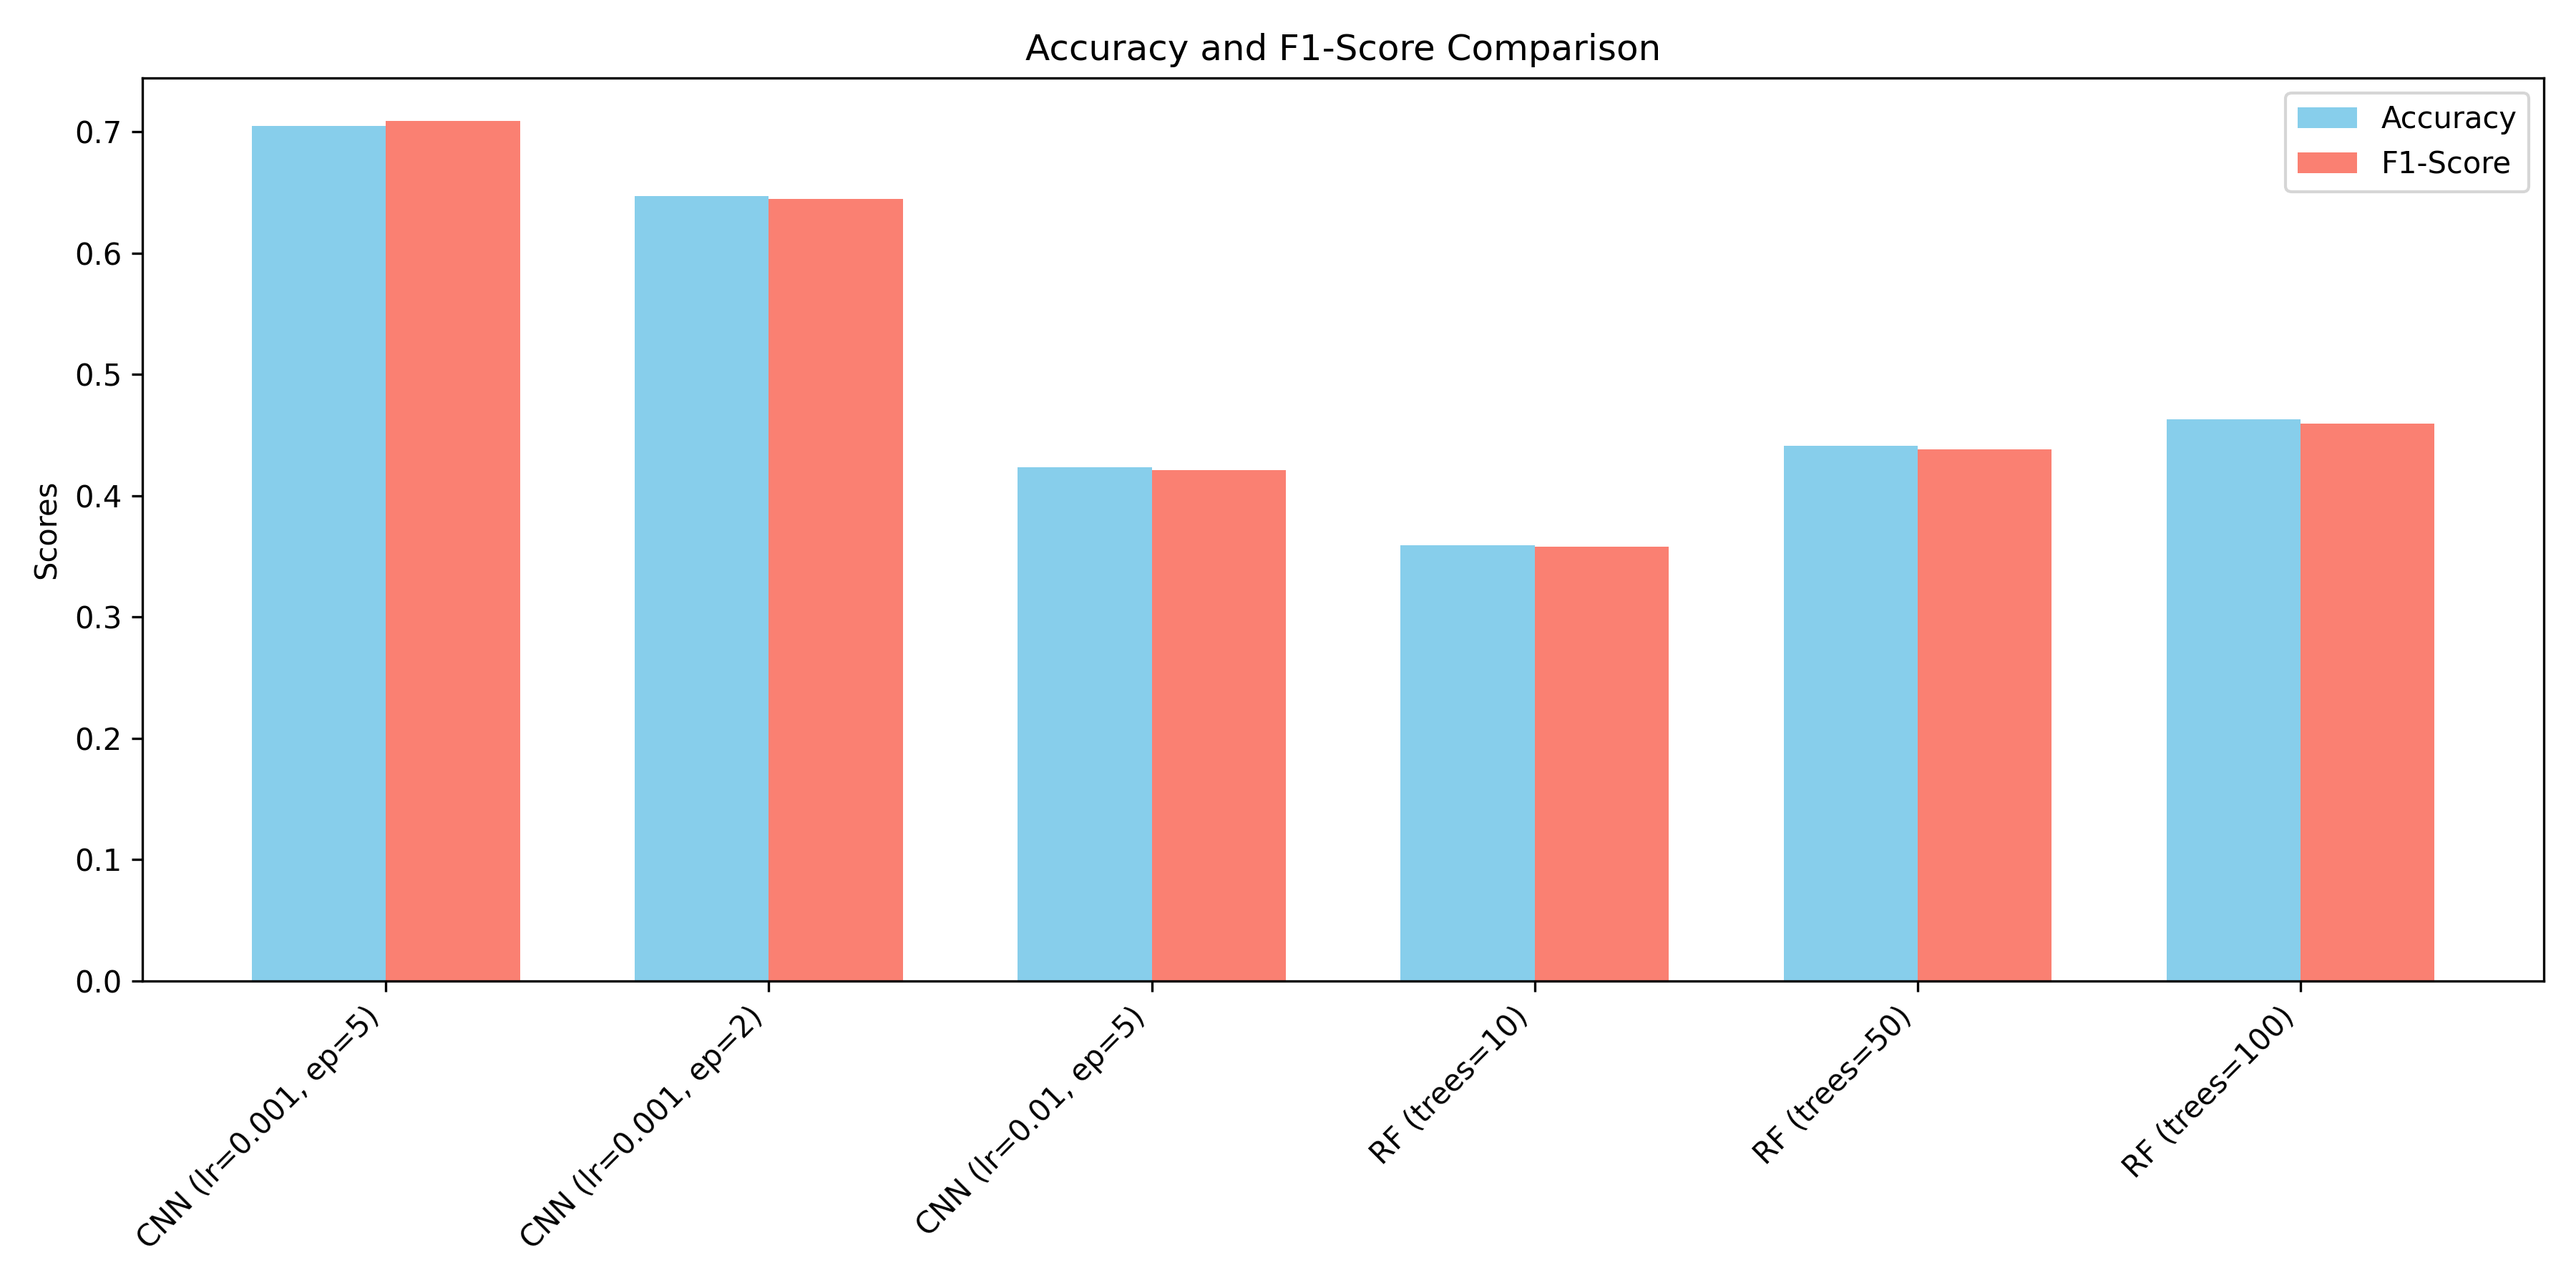
\includegraphics[width=0.85\textwidth]{images/accuracy_vs_f1.png}
    \caption{不同参数配置下模型的 Accuracy 与 F1-Score 对比柱状图}
    \label{fig:accf1}
\end{figure}

\begin{figure}[H]
    \centering
    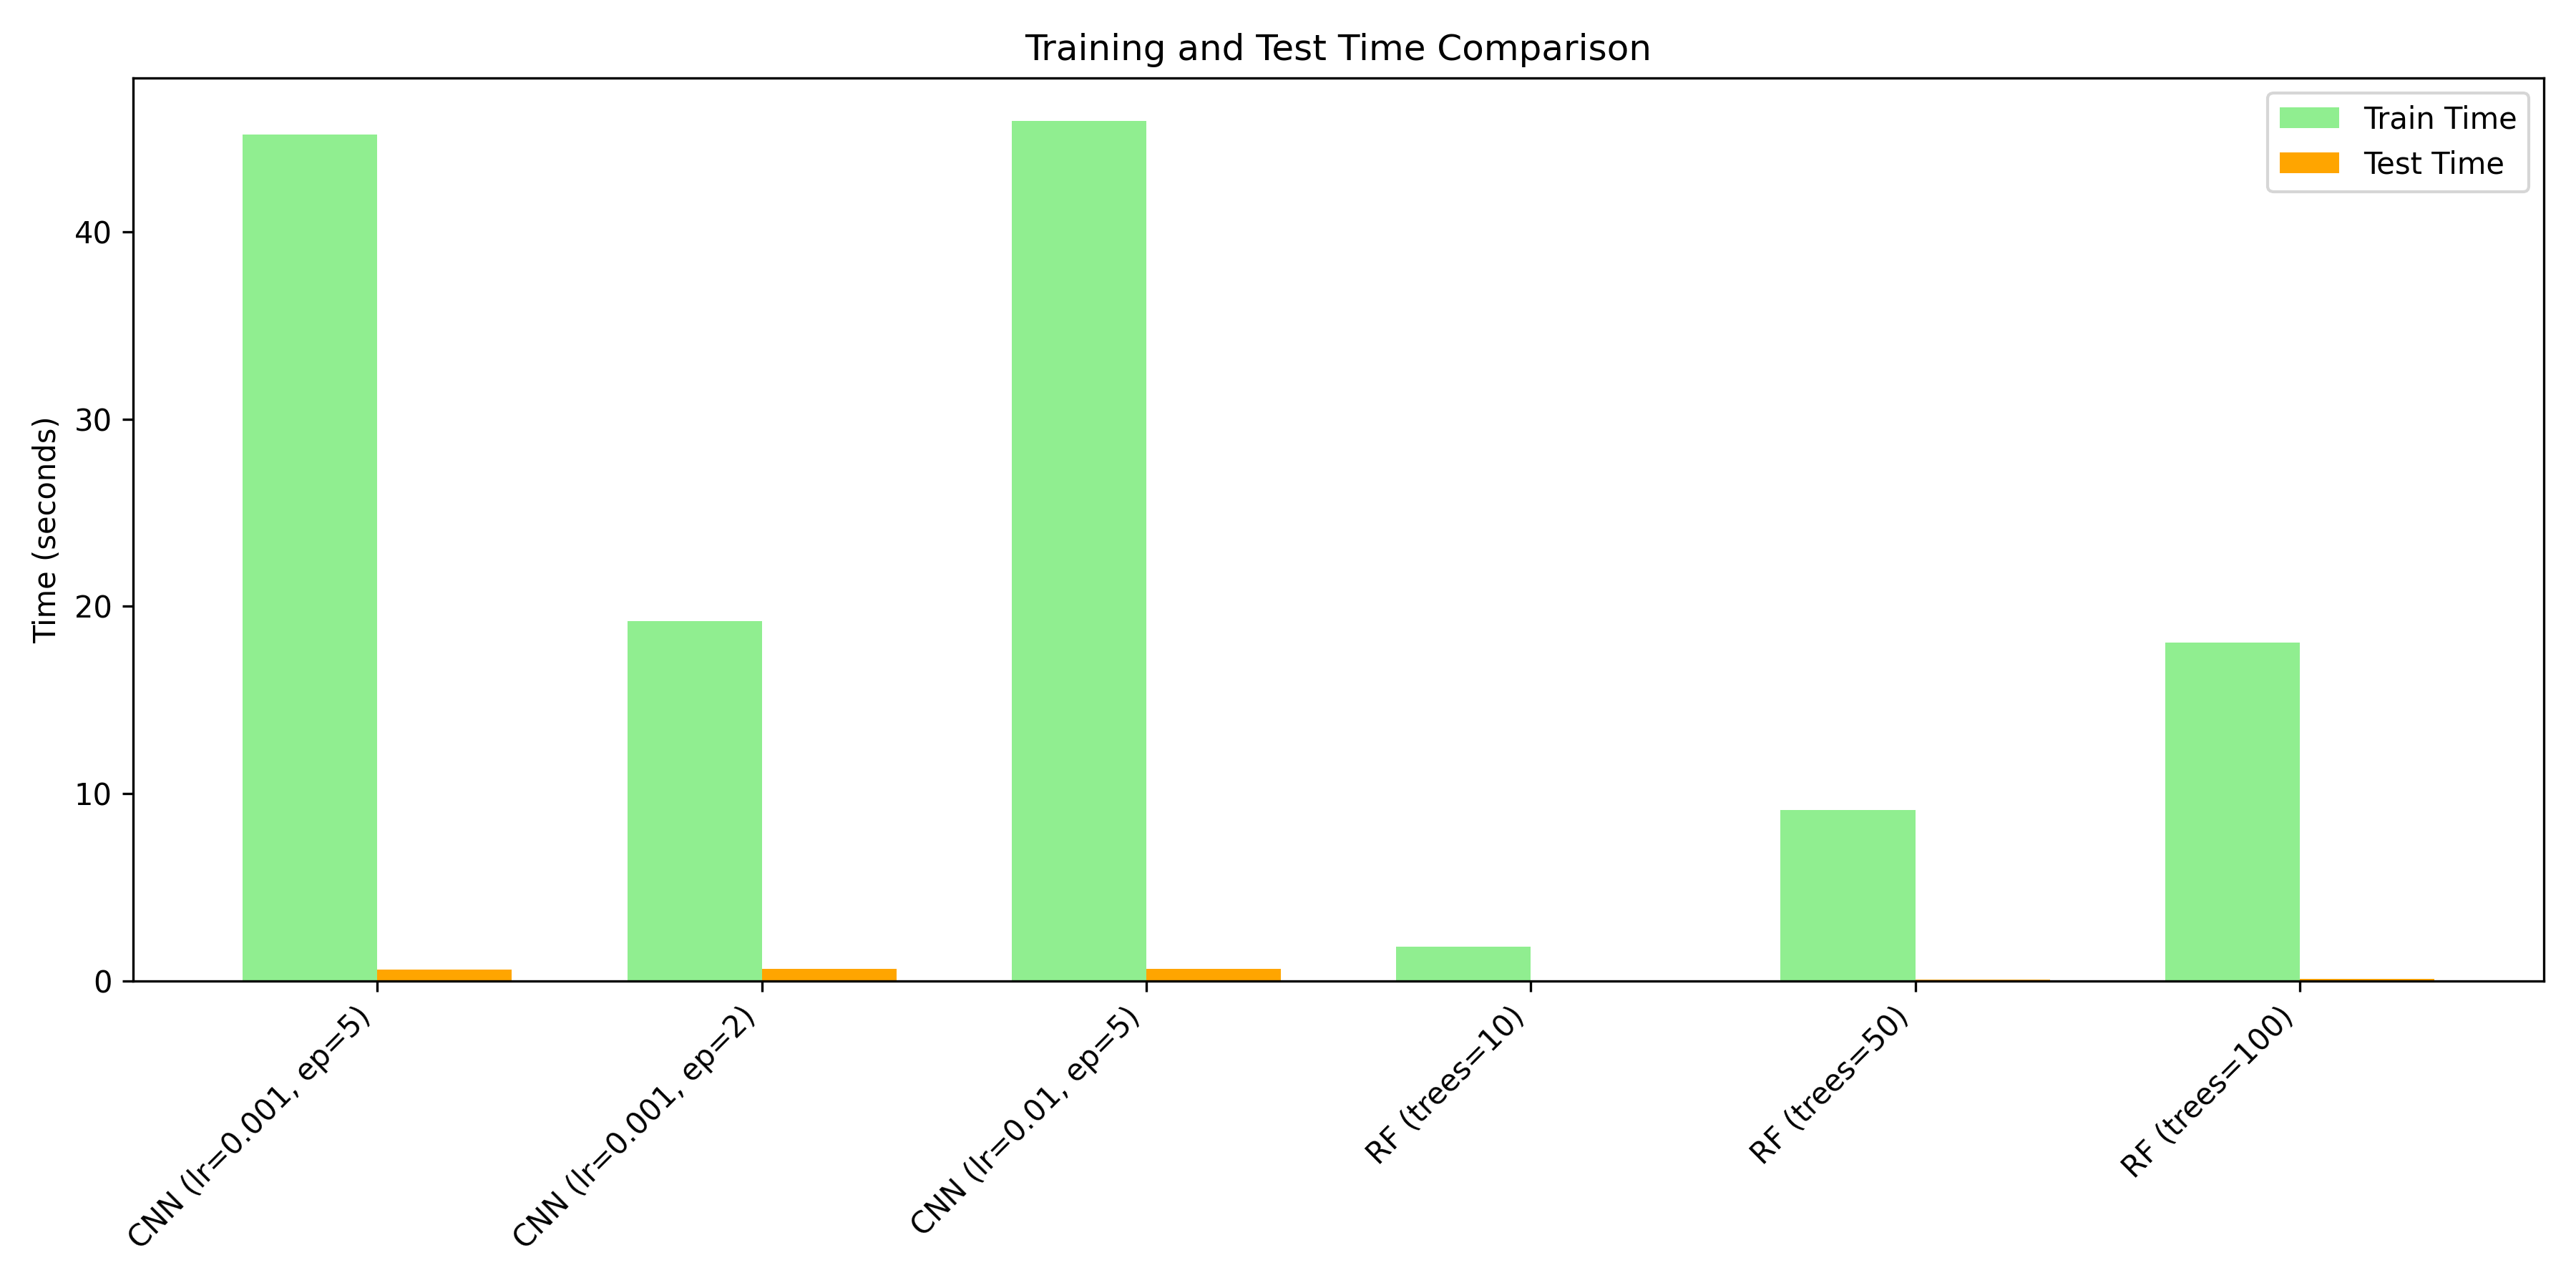
\includegraphics[width=0.85\textwidth]{images/time_comparison.png}
    \caption{不同参数配置下模型的训练时间与测试时间（秒）对比柱状图}
    \label{fig:times}
\end{figure}

\section{总结}
本实验成功完成了基于 CIFAR-10 数据集的两种类别代表性算法对比：
\begin{itemize}
    \item \textbf{性能表现：} 针对高维度且含局部空间特征图像（CIFAR-10），CNN 通过卷积核可以极好地进行空间特征提取，在最终精度上（$\sim 70\%$）压倒性地胜过了仅把像素独立视作特征对待的随机森林系列（上限 $\sim 46\%$）。
    \item \textbf{效率博弈：} 虽然深度模型获得更佳的准确度和 F1 Score，其训练时间负担更重。相较而言，RF 有极低且稳定的推流耗时开销。
    \item \textbf{参数调优：} CNN 高度依赖有效的超参设定，过高学习率会引发学习过程震荡甚至坍塌。而随机森林尽管调参容易（随 $n\_estimators$ 增加性能有预期收敛的稳步提升），但缺乏表达复杂空间联系的模型容量。
\end{itemize}

\paragraph{可改进方向}
未来可尝试更深的 CNN 结构、引入数据增强（随机裁剪、翻转）与学习率调度策略，进一步提升模型泛化能力。同时可使用更强的传统模型（如梯度提升树）验证在图像任务上的上限。

\section*{附录：实验源代码}
\subsection*{A.1 主要源码：\texttt{main.py}}
\begin{lstlisting}
import torch
import torch.nn as nn
import torch.optim as optim
import torchvision
import torchvision.transforms as transforms
from sklearn.ensemble import RandomForestClassifier
from sklearn.metrics import accuracy_score, precision_score, recall_score, f1_score
import time
import numpy as np
import argparse

# ----------------- Part 1: PyTorch CNN ----------------- #
class SimpleCNN(nn.Module):
    def __init__(self):
        super(SimpleCNN, self).__init__()
        # Standard CNN for 32x32 images (CIFAR-10)
        self.conv1 = nn.Conv2d(3, 16, kernel_size=3, padding=1)
        self.relu1 = nn.ReLU()
        self.pool1 = nn.MaxPool2d(2, 2)
        self.conv2 = nn.Conv2d(16, 32, kernel_size=3, padding=1)
        self.relu2 = nn.ReLU()
        self.pool2 = nn.MaxPool2d(2, 2)
        self.fc1 = nn.Linear(32 * 8 * 8, 256)
        self.relu3 = nn.ReLU()
        self.fc2 = nn.Linear(256, 10)

    def forward(self, x):
        x = self.pool1(self.relu1(self.conv1(x)))
        x = self.pool2(self.relu2(self.conv2(x)))
        x = x.view(-1, 32 * 8 * 8)
        x = self.relu3(self.fc1(x))
        x = self.fc2(x)
        return x

def run_cnn(lr=0.001, epochs=5, subset_ratio=1.0):
    print(f"\n--- Running CNN with lr={lr}, epochs={epochs} ---")
    
    transform = transforms.Compose([
        transforms.ToTensor(),
        transforms.Normalize((0.5, 0.5, 0.5), (0.5, 0.5, 0.5))
    ])

    trainset = torchvision.datasets.CIFAR10(root='./data', train=True, download=True, transform=transform)
    testset = torchvision.datasets.CIFAR10(root='./data', train=False, download=True, transform=transform)
    
    if subset_ratio < 1.0:
        train_size = int(len(trainset) * subset_ratio)
        trainset = torch.utils.data.Subset(trainset, range(train_size))
        test_size = int(len(testset) * subset_ratio)
        testset = torch.utils.data.Subset(testset, range(test_size))

    trainloader = torch.utils.data.DataLoader(trainset, batch_size=64, shuffle=True)
    testloader = torch.utils.data.DataLoader(testset, batch_size=64, shuffle=False)

    device = torch.device("cuda:0" if torch.cuda.is_available() else ("mps" if torch.backends.mps.is_available() else "cpu"))
    print(f"Using device: {device}")
    
    model = SimpleCNN().to(device)
    criterion = nn.CrossEntropyLoss()
    optimizer = optim.Adam(model.parameters(), lr=lr)

    # Training
    model.train()
    start_train_time = time.time()
    for epoch in range(epochs):
        running_loss = 0.0
        for i, data in enumerate(trainloader, 0):
            inputs, labels = data[0].to(device), data[1].to(device)
            optimizer.zero_grad()
            outputs = model(inputs)
            loss = criterion(outputs, labels)
            loss.backward()
            optimizer.step()
            running_loss += loss.item()
        print(f"Epoch {epoch+1}, Loss: {running_loss / len(trainloader):.4f}")
    
    train_time = time.time() - start_train_time
    
    # Testing
    model.eval()
    all_preds = []
    all_labels = []
    
    start_test_time = time.time()
    with torch.no_grad():
        for data in testloader:
            inputs, labels = data[0].to(device), data[1].to(device)
            outputs = model(inputs)
            _, predicted = torch.max(outputs.data, 1)
            all_preds.extend(predicted.cpu().numpy())
            all_labels.extend(labels.cpu().numpy())
            
    test_time = time.time() - start_test_time

    # Metrics
    acc = accuracy_score(all_labels, all_preds)
    prec = precision_score(all_labels, all_preds, average='macro', zero_division=0)
    rec = recall_score(all_labels, all_preds, average='macro', zero_division=0)
    f1 = f1_score(all_labels, all_preds, average='macro', zero_division=0)

    print(f"CNN Results (lr={lr}, epochs={epochs}):")
    print(f"Train Time: {train_time:.2f}s | Test Time: {test_time:.2f}s")
    print(f"Accuracy: {acc:.4f} | Precision: {prec:.4f} | Recall: {rec:.4f} | F1-Score: {f1:.4f}")
    return acc, prec, rec, f1, train_time, test_time

# ----------------- Part 2: Scikit-Learn Random Forest ----------------- #
def run_rf(n_estimators=100, max_depth=None, subset_ratio=1.0):
    print(f"\n--- Running Random Forest with n_estimators={n_estimators}, max_depth={max_depth} ---")
    
    # Random Forest works with 1D feature arrays rather than 3D images
    transform = transforms.Compose([transforms.ToTensor()])
    
    trainset = torchvision.datasets.CIFAR10(root='./data', train=True, download=True, transform=transform)
    testset = torchvision.datasets.CIFAR10(root='./data', train=False, download=True, transform=transform)

    if subset_ratio < 1.0:
        train_size = int(len(trainset) * subset_ratio)
        trainset = torch.utils.data.Subset(trainset, range(train_size))
        test_size = int(len(testset) * subset_ratio)
        testset = torch.utils.data.Subset(testset, range(test_size))

    # Convert to NumPy for sklearn
    trainloader = torch.utils.data.DataLoader(trainset, batch_size=len(trainset), shuffle=False)
    testloader = torch.utils.data.DataLoader(testset, batch_size=len(testset), shuffle=False)

    start_prep = time.time()
    # Loading into memory
    X_train, y_train = next(iter(trainloader))
    X_test, y_test = next(iter(testloader))
    
    # Flatten images ([N, 3, 32, 32] -> [N, 3072])
    X_train = X_train.view(X_train.size(0), -1).numpy()
    X_test = X_test.view(X_test.size(0), -1).numpy()
    y_train = y_train.numpy()
    y_test = y_test.numpy()
    print(f"Data Prep Time: {time.time() - start_prep:.2f}s")

    rf = RandomForestClassifier(n_estimators=n_estimators, max_depth=max_depth, n_jobs=-1, random_state=42)
    
    # Training
    start_train_time = time.time()
    rf.fit(X_train, y_train)
    train_time = time.time() - start_train_time

    # Testing
    start_test_time = time.time()
    y_pred = rf.predict(X_test)
    test_time = time.time() - start_test_time

    # Metrics
    acc = accuracy_score(y_test, y_pred)
    prec = precision_score(y_test, y_pred, average='macro', zero_division=0)
    rec = recall_score(y_test, y_pred, average='macro', zero_division=0)
    f1 = f1_score(y_test, y_pred, average='macro', zero_division=0)

    print(f"RF Results (trees={n_estimators}, max_depth={max_depth}):")
    print(f"Train Time: {train_time:.2f}s | Test Time: {test_time:.2f}s")
    print(f"Accuracy: {acc:.4f} | Precision: {prec:.4f} | Recall: {rec:.4f} | F1-Score: {f1:.4f}")
    return acc, prec, rec, f1, train_time, test_time

if __name__ == "__main__":
    import os
    import pandas as pd
    import matplotlib.pyplot as plt

    parser = argparse.ArgumentParser()
    parser.add_argument('--subset', type=float, default=1.0, help="Ratio of data to use (e.g., 0.1 for 10%% to speed up tests)")
    args = parser.parse_args()

    # Create result directory
    os.makedirs('result', exist_ok=True)

    print("=== CIFAR-10 Classification Comparison ===")
    
    results = []

    # 1. Compare CNN parameters
    print("\n[Evaluating CNN Configurations]")
    for lr, epochs in [(0.001, 5), (0.001, 2), (0.01, 5)]:
        acc, prec, rec, f1, train_time, test_time = run_cnn(lr=lr, epochs=epochs, subset_ratio=args.subset)
        results.append({
            'Model': f'CNN (lr={lr}, ep={epochs})',
            'Algorithm': 'CNN',
            'Accuracy': acc,
            'Precision': prec,
            'Recall': rec,
            'F1-Score': f1,
            'Train Time(s)': train_time,
            'Test Time(s)': test_time
        })
    
    # 2. Compare RF parameters
    print("\n[Evaluating RF Configurations]")
    for n_est in [10, 50, 100]:
        acc, prec, rec, f1, train_time, test_time = run_rf(n_estimators=n_est, max_depth=None, subset_ratio=args.subset)
        results.append({
            'Model': f'RF (trees={n_est})',
            'Algorithm': 'RF',
            'Accuracy': acc,
            'Precision': prec,
            'Recall': rec,
            'F1-Score': f1,
            'Train Time(s)': train_time,
            'Test Time(s)': test_time
        })
        
    # Create a DataFrame
    df = pd.DataFrame(results)
    
    # Print the table
    print("\n=== Final Results Table ===")
    print(df.to_string(index=False))
    
    # Save the table outputs
    df.to_csv('result/metrics_comparison.csv', index=False)
    df.to_markdown('result/metrics_comparison.md', index=False)
    
    # Visualization
    print("\nSaving visualizations to 'result' folder...")
    
    # 1. Accuracy & F1-Score Plot
    fig, ax = plt.subplots(figsize=(12, 6))
    x = np.arange(len(df['Model']))
    width = 0.35
    
    ax.bar(x - width/2, df['Accuracy'], width, label='Accuracy', color='skyblue')
    ax.bar(x + width/2, df['F1-Score'], width, label='F1-Score', color='salmon')
    
    ax.set_ylabel('Scores')
    ax.set_title('Accuracy and F1-Score Comparison')
    ax.set_xticks(x)
    ax.set_xticklabels(df['Model'], rotation=45, ha='right')
    ax.legend(loc='upper right')
    plt.tight_layout()
    plt.savefig('result/accuracy_vs_f1.png', dpi=300)
    plt.close()
    
    # 2. Training Time vs Test Time Plot
    fig, ax = plt.subplots(figsize=(12, 6))
    ax.bar(x - width/2, df['Train Time(s)'], width, label='Train Time', color='lightgreen')
    ax.bar(x + width/2, df['Test Time(s)'], width, label='Test Time', color='orange')
    
    ax.set_ylabel('Time (seconds)')
    ax.set_title('Training and Test Time Comparison')
    ax.set_xticks(x)
    ax.set_xticklabels(df['Model'], rotation=45, ha='right')
    ax.legend(loc='upper right')
    plt.tight_layout()
    plt.savefig('result/time_comparison.png', dpi=300)
    plt.close()

    print("Done! Visualizations and tables are saved in 'result/' directory.")
\end{lstlisting}

\subsection*{A.2 运行命令}

\begin{verbatim}
# 完整训练与评估
python main.py

# 使用子集快速验证
python main.py --subset 0.1
\end{verbatim}


\end{document}
